\documentclass{article}
\usepackage{amsmath}
\usepackage{amsfonts}
\usepackage{graphicx}
\usepackage{url}
\usepackage[slovene]{babel}

\author{Lucija Fekonja}
\title{Poročilo o implementaciji detektorja QRS kompleksov}
% \affiliation{Univerza v Ljubljani, Fakulteta za računalništvo in informatiko}


\begin{document}
\selectlanguage{slovene}

    \maketitle

    \begin{abstract}
        V sklopu prve seminarske naloge pri predmetu Obdelava biomedicinskih signalov in slik smo
        implementirali detektor QRS kompleksov. V našem primeru smo to naredili z uporabo dveh elektrod, 
        pri čemer smo sledili pristopu, predstavljenemu v članku \emph{A QRS Complex Detection Algorithm Using 
        Electrocardiogram Leads} \cite{article}. Razviti detektor smo nato evalvirali na podatkovnih bazah MIT/BIH Arrhythmia Database
        in na Long Term ST Database, pri čemer smo analizirali 
        njegovo občutljivost in natančnost pri zaznavanju QRS kompleksov v elektrokardiogramih.
    \end{abstract}

    \section{Uvod}
    V okviru seminarske naloge smo implementirali algoritem za zaznavanje srčnega utripa, 
    ki temelji na združitvi dveh detekcijskih modulov. Za izboljšanje robustnosti detektorja smo 
    uporabili večkanalni elektrokardiogram (EKG), kar nam omogoča zmanjšanje vpliva na delovanje 
    detektorja v primeru, da ima en izmed kanalov signale nizke kakovosti, kot so nizka amplituda 
    ali šum. 

    Detektor je sestavljen iz treh ključnih delov: filtra, glavnega detekcijskega modula ter 
    sekundarnega detekcijskega modula, ki se aktivira v primeru, ko glavni modul ne more jasno definirati, 
    ali se je srčni utrip zgodil ali ne. Implementacijo smo izvedli v okolju MATLAB, pri čemer smo uporabili 
    podatke iz MIT-BIH baze in LTSTDB. Za vsak zapis smo pridobili \emph{X.hea}, \emph{X.dat} in \emph{X.atr} datoteke, ki smo jih nato 
    pretvorili v MATLAB formate s pomočjo ukaza \textbf{wfdb2mat -i X}. S tem smo ustvarili \emph{Xm.mat} datoteko, ki smo 
    jo integrirali v naš detektor srčnega utripa, predstavljen v nadaljevanju poročila.
    
    \section{Metoda}
    V naši metodi detekcije, detektor sprejme dva vhodna signala, $x_1$ in $x_2$. 
    Pred začetkom detekcije vsak signal prestane filtracijo, ki jo izvajamo s pomočjo \path{signal_conditioner.mat}. Absolutne vrednosti 
    filtriranih signalov nato seštejemo. Ta kombiniran signal nato vstopi v glavni detektor, imenovan \path{main_detector.mat}, 
    ki uporablja dva praga za učinkovito zaznavanje QRS kompleksov. QRS kompleks se šteje za zaznanega, če signal 
    v zadnjih $180$ $ms$ preseže prag v dveh do štirih točkah. V primeru, da preseže prag v več kot štirih točkah, 
    smatramo zadnjih $180$ $ms$ za šum in prilagodimo pragove navzgor. Nasprotno, če ni bilo zaznanih presekov, znižamo pragove.

    V primeru zaznanih presekov v le eni točki uporabimo sekundarni detektor, implementiran v datoteki \path{secondary_detector.mat}. 
    Ta detektor deluje na podlagi energijskega signala, ki je izračunan iz že filtriranega signala. 

    \subsection{Pripravljalnik signala}
    Preden lahko signala $x_1$ in $x_2$ uporabimo v detektorju, ju moramo ustrezno prilagoditi. Zato na vsakem
    od njiju najprej uporabimo nizkoprepustni filter
    $$ y(n) = \frac{1}{4} x(n-2) + \frac{1}{2} x(n-1) + \frac{1}{4} x(n) \text{,}$$
    katerega prenosna karakteristika je 
    $$ H(z) = \frac{(1 + z)^2}{4 z^2} \text{.}$$
    Nato signal pošljemo skozi omrežni filter, ki se znebi nepotrebnega šuma. Njegova diferencialna enačba in prenosna funkcija sta
    $$ y(n) = x(n - 2) - 2 \cos \left( \frac{60 \pi}{125} \right) x(n-1) + x(n)\text{,} \qquad H(z) = \frac{1 - 2 \cos \left( \frac{60 \pi}{125} \right) z + z^2}{z^2} \text{.}$$
    Signal pošljemo skozi še zadnji, odvodni filter
    $$ y(n) = x(n) + x(n - 6)\text{,} \qquad H(z) = \frac{1 + z^6}{z^6}\text{.}$$
    Vsi trije filtri so stabilni. Tudi njihov produkt je stabilen, kot je razvidno iz Slike 1. 
    \begin{figure}[h]
        \centering
        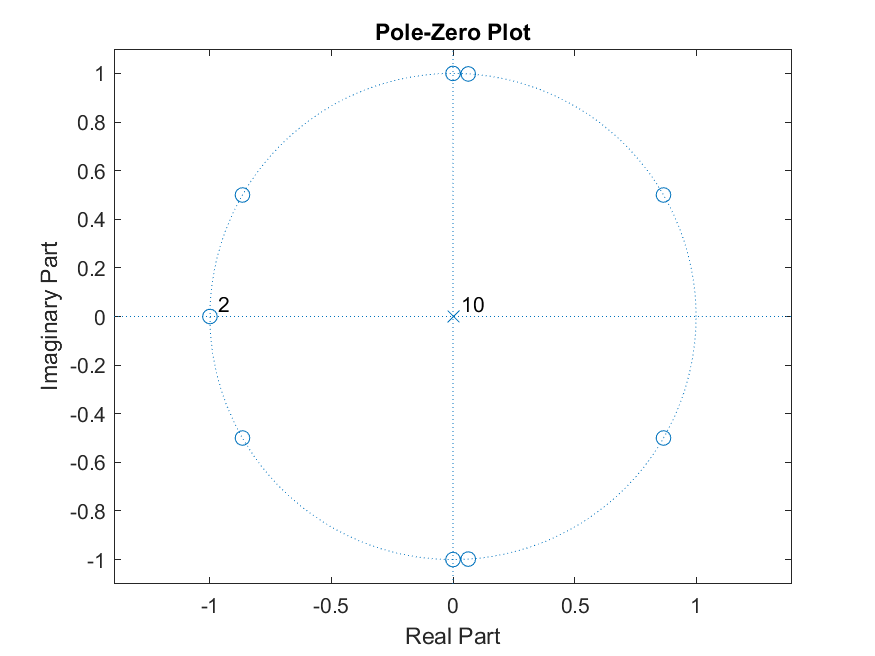
\includegraphics[width=0.4\textwidth]{stabilnost_filtrov.png}
        \caption{Ničle in poli prenosne karakteristike filtra v $z$-ravnini.}
    \end{figure}
    V glavni detektor pošljemo vsoto absolutnih obeh filtriranih signalov. 

    \subsection{Glavni detektor}
    Glavni detektor prejme filtriran signal in oceni, kolikokrat ta preseže detekcijski prag (\emph{DT}). QRS 
    kompleks zazna, če signal v zadnjih $180$ $ms$ preseže \emph{DT} dva do štirikrat. Vrednost \emph{DT} je določena na podlagi 
    baznega praga (\emph{BT}). Postopek določanja \emph{DT} temelji na naslednjih pravilih.
    
    Če je v zadnjih $180$ $ms$ prišlo do več kot štirih presečišč med signalom in \emph{DT}, smo v območju šuma. V tem primeru 
    dvignemo \emph{BT} in $DT$ na 
    \begin{align*}
        BT &= 1.5 \times BT \\
        DT &= \max(0.5 \times \max(peak), BT) \text{,}
    \end{align*}
    kjer je $peak$ maksimum zadnjih $180$ $ms$ signala. 

    Če signal ni presegel praga v $180$ $ms$, se mora ustrezno znižati na polovico vrednosti \emph{BT}. Če presečišča ni $360$ $ms$,
    se \emph{DT} zniža na višjo od vrednosti $0.75 \times DT$ oziroma $0.5 \times BT$.

    Ko je QRS kompleks zaznan, se \emph{BT} in $DT$ povečata:
    \begin{align*}
        BT &= 0.75 \times BT + 0.25 \times (peak) \text{,} \\
        DT &= \max(0.5 \times (peak), BT) \text{.}
    \end{align*}
    Kot točko, v kateri je QRS kompleks zaznan, smo označili prvi indeks, pri katerem
    je prišlo do presečišča, v kolikor detektor ni zaznal srčnega utripa vsaj $180$ $ms$ pred tem.

    V vseh ostalih primerih se \emph{BT} in \emph{DT} ohranita.

    \subsection{Sekundarni detektor}
    V glavnem detektorju smo izpusti možnost, da signal seka prag natanko enkrat. V tem primeru se uporabi sekundarni detektor, ki sprejme 
    signal filtriran z energijskim filtrom. Ta je implementiran v \path{energy_filter.mat}. Enak je povprečju 
    kvadratov zadnjih osmih sekund. Energijski signal nato primerjamo z detekcijskim pragom energijskega signala ($ET$).
    
    Kadar signal preseže $ET$, se slednji zviša na
    \begin{equation}
        \label{eqn:ET}
        ET = 4 \times ( 0,75 \times ET + 0,5 \times QRS (peak)) \text{.}
    \end{equation}
    Cilj je, da detektor ne zazna utripa nadaljnjih $200$ $ms$. Če zazna, se prag ponovno dvigne, kot je opisano 
    zgoraj \ref{eqn:ET}, in indeks, ki ga bomo dodali kot točko QRS kompleksa, se spremeni iz prejšnjega presečišča 
    na trenutno presečišče. Ta postopek se ponovi. Po $200$ $ms$ brez novega presečišča se $ET$ zniža na petino svoje 
    vrednosti.
    
    Če detektor ni zaznal utripa $1$ $s$, se $ET$ zniža na polovico, v vseh ostalih primerih pa ostane enak. 

    Glavni detektor ne shrani vseh točk, v katerih bi lahko bil QRS kompleks. Sekundarni detektor dopolnjije glavnega tako, 
    da v množico vseh QRS kompleksov zaznanih z glavnim detektorjem doda tiste QRS komplekse zaznane s sekundarnim, katerih razlika 
    od vseh je večja od neke določene vrednosti. V našem primeru več kot $\frac{2 \times F_s}{5}$ vzorcev.

    \section{Rezultati}
    Detektor smo testirali na bazah MIT/BIH Arrhythmia Database in Long Term ST Database. Algoritem smo evalvirali glede na občutljivost \emph{Se} in 
    natančnost \emph{P+}. Na MIT/BIT bazi smo dobili naslednje rezultate:
    \begin{align*}
        TP &= Nn + Vn + Fn = 80624 + 5520 + 8507 = 94651 \\
        FN &= No + Vo + Fo = 12788 + 1716 + 339 = 14843 \\
        FP &= On = 12297
    \end{align*}
    Občutljivost je delež pravilno zaznanih QRS kompleksov med vsemi dejanskimi QRS kompleksi: $Se = \frac{TP}{TP + FN} = 86.4\%$.
    Natančnost je delež vseh pravilno zaznanih QRS kompleksov med vsemi zaznanimi QRS kompleksi: $P+ = \frac{TP}{TP + FP} = 88.5\%$.

    Na LTSTDB bazi smo dobili naslednje rezultate:
    \begin{align*}
        TP &= Nn + Vn + Fn = 6884791 + 51550 + 311 = 6936652 \\
        FN &= No + Vo + Fo = 1939466 + 21373 + 289 = 1961128 \\
        FP &= On = 1438796
    \end{align*}
    Občutljivost je delež pravilno zaznanih QRS kompleksov med vsemi dejanskimi QRS kompleksi: $Se = \frac{TP}{TP + FN} = 78.0\%$.
    Natančnost je delež vseh pravilno zaznanih QRS kompleksov med vsemi zaznanimi QRS kompleksi: $P+ = \frac{TP}{TP + FP} = 82.8\%$.



    \section{Zaključek}
    V implementaciji detektorja QRS kompleksov smo združili signale dveh elektrod, kar se izkaže za izjemno koristno v primerih, ko 
    je eden od signalov slab zaradi šuma ali nizke amplitude. Na začetku smo oba signala filtrirali s filtrom, ki je zmanjšal šum in 
    nihanje ničelnega nivoja ter hkrati ojačal frekvence v območju med $9$ in $30$ $Hz$. Uporaba obeh signalov omogoča robustnejšo 
    detekcijo srčnih utripov in izboljšuje zanesljivost celotnega sistema.

    Detektor deluje s pomočjo dveh detekcijskih modulov. Glavni detektor je bil izbran zaradi svoje učinkovitosti in enostavnosti. 
    Njegov pristop, kjer se vsako prečkanje praga obravnava kot potencialni trenutek srčnega utripa, omogoča hitrejšo detekcijo srčnih 
    utripov. Prilagodljivost sistema je dosežena s hitrim prilagajanjem obeh pragov glede na amplitudo signala. Zvišanje praga ob zaznavi 
    šuma prispeva k izločitvi intervalov, ki so posledica šuma, kar povečuje natančnost detekcije.

    Sekundarni detektor se uporablja v primerih, ko glavni detektor ne zazna srčnega utripa. Uporablja energijski signal za boljše 
    razlikovanje med QRS kompleksom in motnjami, kot so šum in nihanje ničelnega nivoja. Rezultat uporabe sekundarnega detektorja 
    je zmanjšanje lažno negativnih rezultatov, kar dodatno povečuje zanesljivost sistema.

    Prva šibka točka se pojavlja, ko oba vhodna signala vsebujeta šum. V tem primeru detektor deluje podobno kot detektor z enim 
    samim vhodnim signalom. Druga pomembna pomanjkljivost naše implementacije je, da detektor ne deluje v realnem času in je 
    prepočasen. Za vsak posamezen signal iz MIT/BIT baze potrebuje povprečno eno sekundo, medtem ko za signal iz baze LTSTDB 
    porabi celo minuto in pol. Časovna učinkovitost bi se lahko izboljšala z uporabo premikajočega se okna namesto preverjanja 
    vseh točk vhodnega signala, vendar bi to morda kompromitiralo občutljivost in natančnost detektorja.

    \begin{thebibliography}{9}
        \bibitem{article}
        JCTB Moraes (1986) \emph{A QRS Complex Detection Algorithm Using Electrocardiogram Leads}, Escola Politdcnica da Universidade de S5o Paulo, SBo Paulo, Brazil.
    \end{thebibliography}

\end{document}